% --- [ Interval Method ] ------------------------------------------------------

\subsection{Interval Method}
\label{sec:interval_method}

% Reducible control flow graphs are reducible by intervals.

The interval method is a control flow recovery method which identifies the loops in a control flow graph $G$ and determines their type based on the back edges of the intervals of $G$. The nesting levels of loops are determined based on the derived sequence of graphs $G^1 \dots G^n$.

\todo{TODO: add review \cite{structuring_decompiled_graphs}}

% From Cifuentes' Since the underlying structure of the graph is not modified, functional and semantical equivalence is preserved by this method.

% From Cifuentes' about her own algorithm: If the graph cannot be structured with the predefined set of structures, goto jumps are used. These conditions ensure functional and semantical equivalence between the original and final graph.


% From Cifuentes' Loops are detected by the presence of a back-edge.
% From Cifuentes' The type of the loop is detected by checking the header and the last node of the loop.

% TODO: make into a table.

             Header   Latch    Type
Condition    no       no       endless
Condition    yes      no       pre-test
Condition    no       yes      post-test
Condition    yes      yes      pre-test loop with if-then break at the end of the loop body.

% ---> important. Cifuentes' also distinguish "control nodes". I.e. nodes that only transfer control flow. From Cifuentes', to handle Compound conditional branches: But since both B7 and B8 only have a conditional branch instruction, these two conditions could be merged into a compound conditional.

% Cifuentes' definition: A latching node is any node in the interval which has the header node as an immediate successor.

% From Cifuentes' Derived Sequence Construction. G is the first order graph, represented G^1. The second order graph, G^2 , is derived from G^1 by collapsing each interval in G^1 into a node. The immediate predecessors of the collapsed node are the immediate predecessors of the original header node which are not part of the interval. The immediate successors are all the immediate, non-interval successors of the original exit nodes.

 % From Cifuentes' G^n has the property of being a trivial graph (i.e. single node) or an irreducible graph.

% From Cifuentes' The absence of the canonical irreducible graph in a flow graph is enough for the graph to be reducible.

% From Cifuentes' A structured control flow graph: graph that is decomposable into subgraphs with one entry and one or more exits

% From Cifuentes' Unstructured graphs are generated by the unstructured transfer of control of goto statements, that is, a transfer of control in the middle of a structured graph, which breaks the previously structured graph into an unstructured one since there is more than one entry into this subgraph. Unstructuredness can also be introduced by the optimization phase of the compiler when code motion is performed (i.e. code is moved).

% From Cifuentes' The follow node of a structured or unstructured loop is the first node that is reached from the exit of the loop.

% Loop structuring.
% From Cifuentes' As pointed out by Hecht in [Hec77], the representation of a loop by means of cycles is too fine a representation since loops are not necessarily properly nested or disjoint. The use of strongly connected components as loops is too coarse a representation as there is no nesting order. The use of strongly connected regions does not provide a unique cover of the graph, and does not cover the entire graph. Finally, the use of intervals does provide a representation that satisfies the abovementioned conditions: one loop per interval, and a nesting order provided by the derived sequence of graphs.

% Loop structuring from Cifuentes'
% Once a loop has been found, the type of loop (e.g. pre-tested, post-tested, endless) is determined according to the type of header and latching nodes.
% Also, the nodes that belong to the loop are flagged as being so, in order to prevent nodes from belonging to two different loops, such as in overlapping, or multientry loops.
%s
% an algorithm to find loops is as follows: each header of an interval in G 1 is checked for having a back-edge from a latching node that belong to the same interval.
%
% If this happens, a loop has been found, so its type is determined, and the nodes that belong to it are marked.
%
% Next, the intervals of G^2 , I^2 are checked for loops, and the process is repeated until intervals in I^n have been checked.
%
% Whenever there is a potential loop (i.e. a header of an interval that has a predecessor with a back-edge) that has its header or latching node marked as belonging to another loop, the loop is disregarded as it belongs to an unstructured loop.
%
% In this case, an extra condition is needed to be satisfied, and that is, that the nodes belong to the same interval, since the interval header (i.e. x) dominates all nodes of the interval, and in a loop, the loop header node dominates all nodes of the loop. If a node belongs to a different interval, it is not dominated by the loop header node, thus it cannot belong to the same loop.
%
% From Cifuentes' In other words, a node n belongs to the loop induced by (y, x) if it belongs to the same interval (i.e. it is dominated by x), and its order (i.e. reverse postorder number) is greater than the header node and lesser than the latching node (i.e. it is a node from the “middle” of the loop).

% From Cifuentes' the node that has a greater reverse postorder numbering needs to be analyzed first since it was last visited first in the depth first search traversal.

% Cifuentes' short-circuit evaluation of compound Boolean conditions. In these languages, the generated control flow graphs for these conditional expressions become unstructured since an exit can be performed as soon as enough conditions have been checked and determined the expression is true or false as a whole.
%
% ---> essnetially condition node ---> 3. Node y has a unique instruction, a conditional jump (jcond) high-level instruction.
%
% The algorithm to structure compound conditionals makes use of a traversal from top to bottom of the graph, as the first condition in a compound conditional expression is higher up in the graph.

% Cifuentes' N-way conditionals are structured in a similar way to 2-way conditionals. Nodes are traversed from bottom to top of the graph in order to find nested n-way conditionals first, followed by the outer ones.
%
% Candidate follow nodes are all nodes that have the header node 1 as immediate dominator, and that are not successors of this node.

% Cifuentes' determine the entry and exit (i.e. header and follow) nodes of subgraphs that represent high-level loops, n-way, and 2-way structures.
%
% These algorithms cannot be applied in a random order since they do not form a finite Church-Rosser system.
%
% Order: structure n-way conditionals, followed by loop structuring, and 2-way conditional structuring last.
%
% Loops are structured before 2-way conditionals to ensure the Boolean condition that form part of pre-tested or post-tested loops is part of the loop, rather than the header of a 2-way conditional subgraph.

% Cifuentes' How the canonicl irreducible graph is structured: Since the graph is irreducible, there is no loop that is contained entirely in an interval, therefore, the loop structuring algorithm determines that there are no natural loops as such. When structuring 2-way conditionals, the conditional at node 1 is determined to have the follow node 3, since this node is reached from both paths from the header node and has a greater numbering than node 2.

% Cifuentes' As pointed out by Hecht in [Hec77], the representation of a loop by means of cycles is too fine a representation since loops are not necessarily properly nested or disjoint. The use of strongly connected components as loops is too coarse a representation as there is no nesting order. The use of strongly connected regions does not provide a unique cover of the graph, and does not cover the entire graph. Finally, the use of intervals does provide a representation that satisfies the abovementioned conditions: one loop per interval, and a nesting order provided by the derived sequence of graphs

% Cifuentes' each header of an interval in G^i is checked for having a back- edge from a latching node that belong to the same interval.

% Cifuentes' Whenever there is a potential loop (i.e. a header of an interval that has a predecessor with a back-edge) that has its header or latching node marked as belonging to another loop, the loop is disregarded as it belongs to an unstructured loop. These loops always generate goto jumps during code generation.

% Cifuentes'  This algorithm finds the loops in the appropriate nesting level, from innermost to outermost loop.

% ~~~ [ Interval ] ~~~~~~~~~~~~~~~~~~~~~~~~~~~~~~~~~~~~~~~~~~~~~~~~~~~~~~~~~~~~~

\subsubsection{Interval}

An interval $I(h)$ with header node $h$ is a maximal single-entry subgraph in which $h$ is the only entry node and all cycles contain $h$ \cite{structuring_algorithm_for_decompilation}. The example illustrated in figure \ref{fig:interval} highlights the unique set of intervals \textbf{I(B1)}, \textbf{I(B6)}, and \textbf{I(B13)} in a control flow graph.

\begin{figure}[htbp]
	\centering
	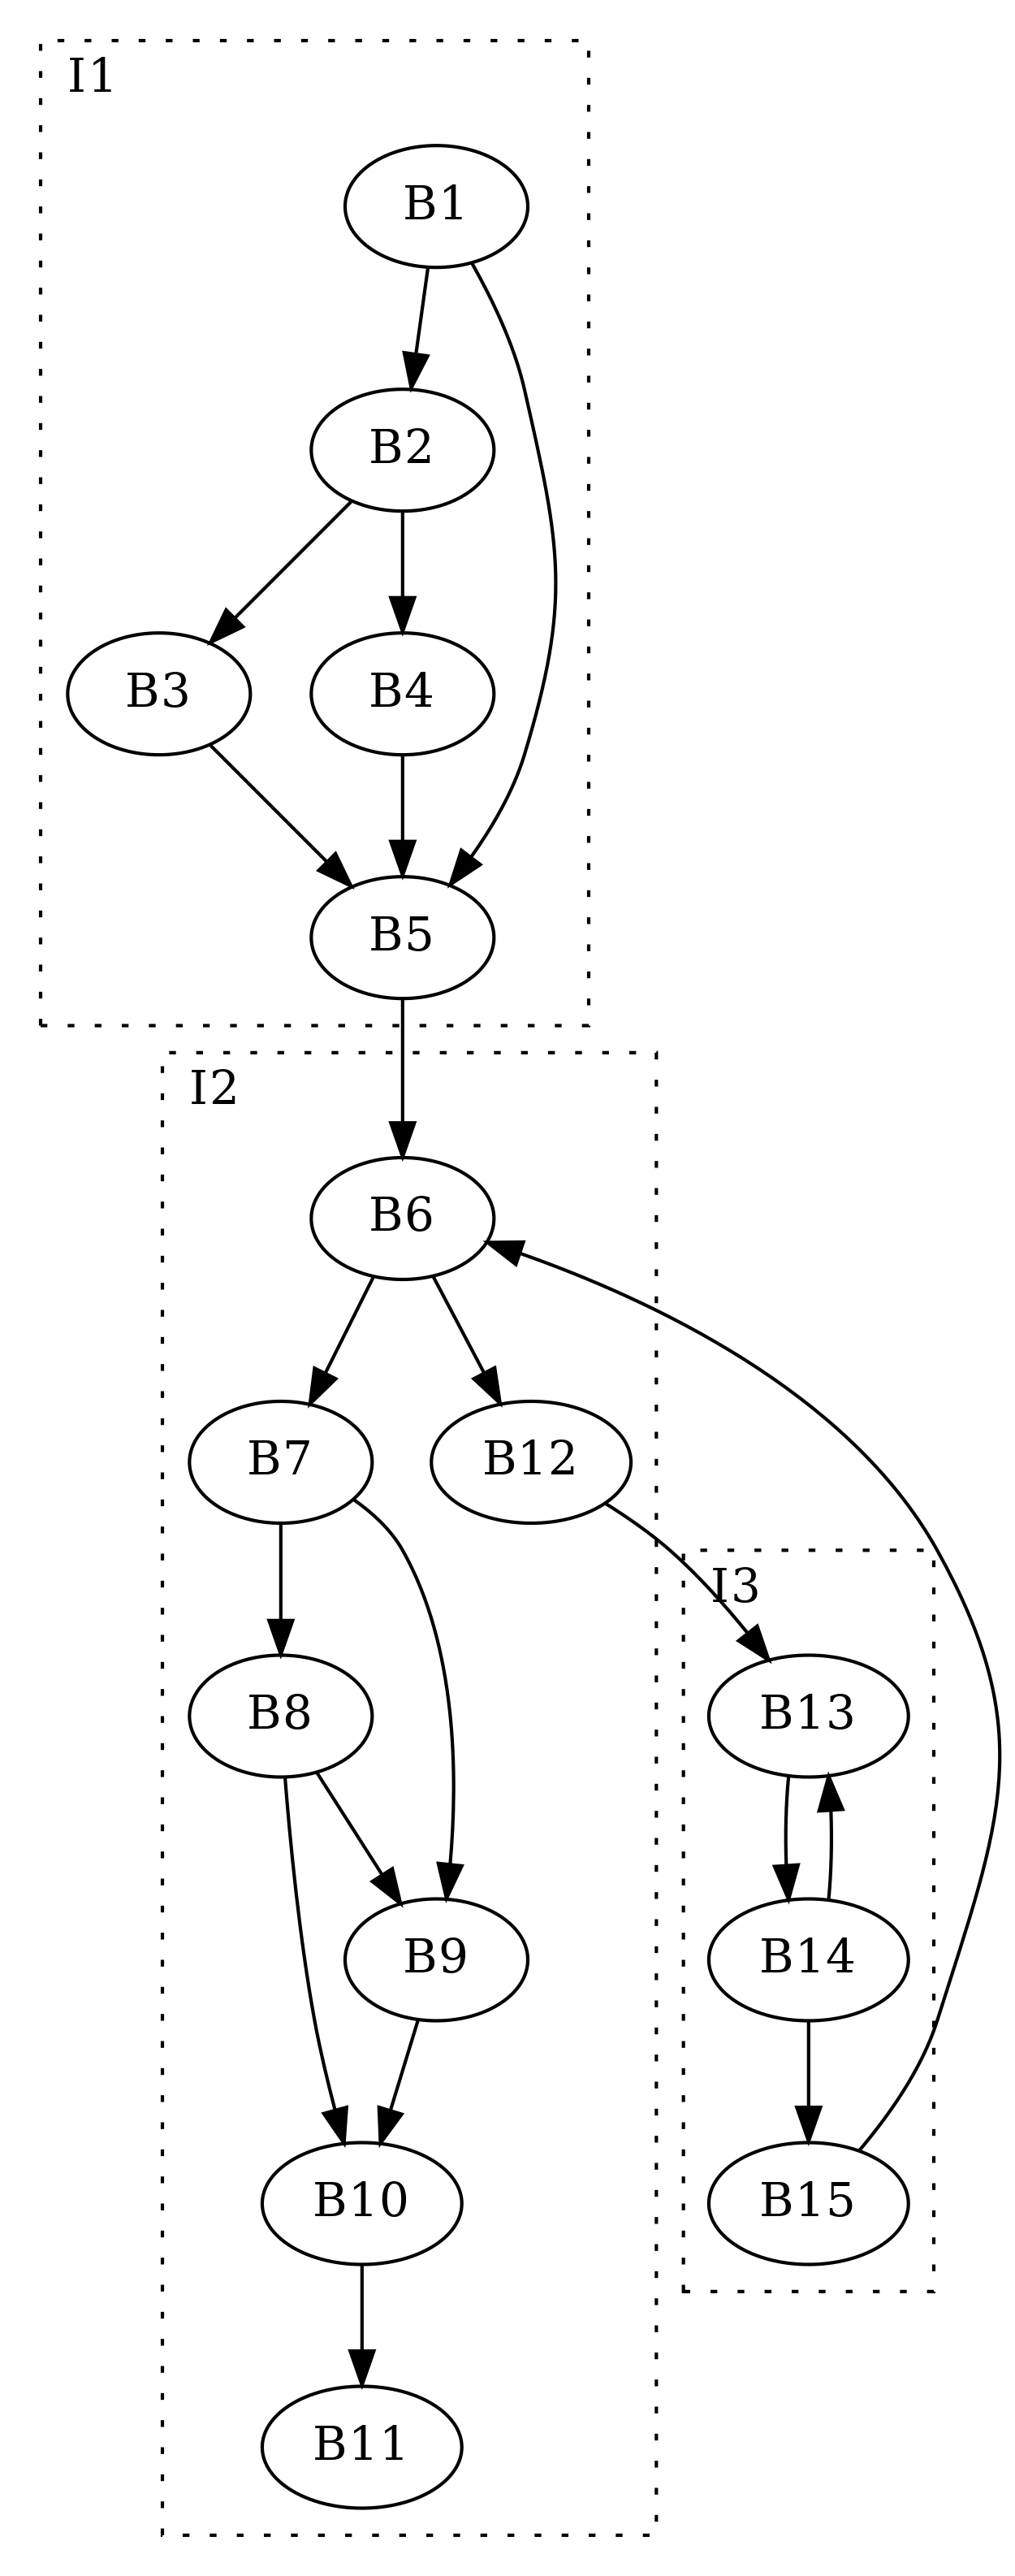
\includegraphics[width=0.3\textwidth]{inc/appendices/vocabulary/interval.png}
	\caption{The intervals \textbf{I1}, \textbf{I2} and \textbf{I3} outlined in a control flow graph; adapted from figure 2 of C. Cifuentes' \textit{Structuring Decompiled Graphs} \cite{structuring_decompiled_graphs}.}
	\label{fig:interval}
\end{figure}

% ~~~ [ Derived Sequence of Graphs G^1...G^n ] ~~~~~~~~~~~~~~~~~~~~~~~~~~~~~~~~~

\subsubsection{Derived Sequence of Graphs}

Given a control flow graph $G$ a derived sequence of graphs, $G^1 \dots G^n$, may be constructed by collapsing intervals. The first order graph $G^1 = G$. The second order graph $G^2$ is obtained by collapsing each interval in $G^1$ into a node. The node of a collapsed interval $I(h)$ has incoming edges from the immediate predecessors of the header node $h$ not part of the interval, and outgoing edges to the immediate successors of the exit nodes of $I(h)$ not part of the interval. The intervals of $G^2$ are collapsed and the process is repeated until $G^n$ is a single node or an irreducible graph; as illustrated in figure \ref{fig:derived_sequence_of_graphs}.

\begin{figure}[htbp]
	\centering
	\begin{subfigure}[b]{0.30\textwidth}
		\centering
		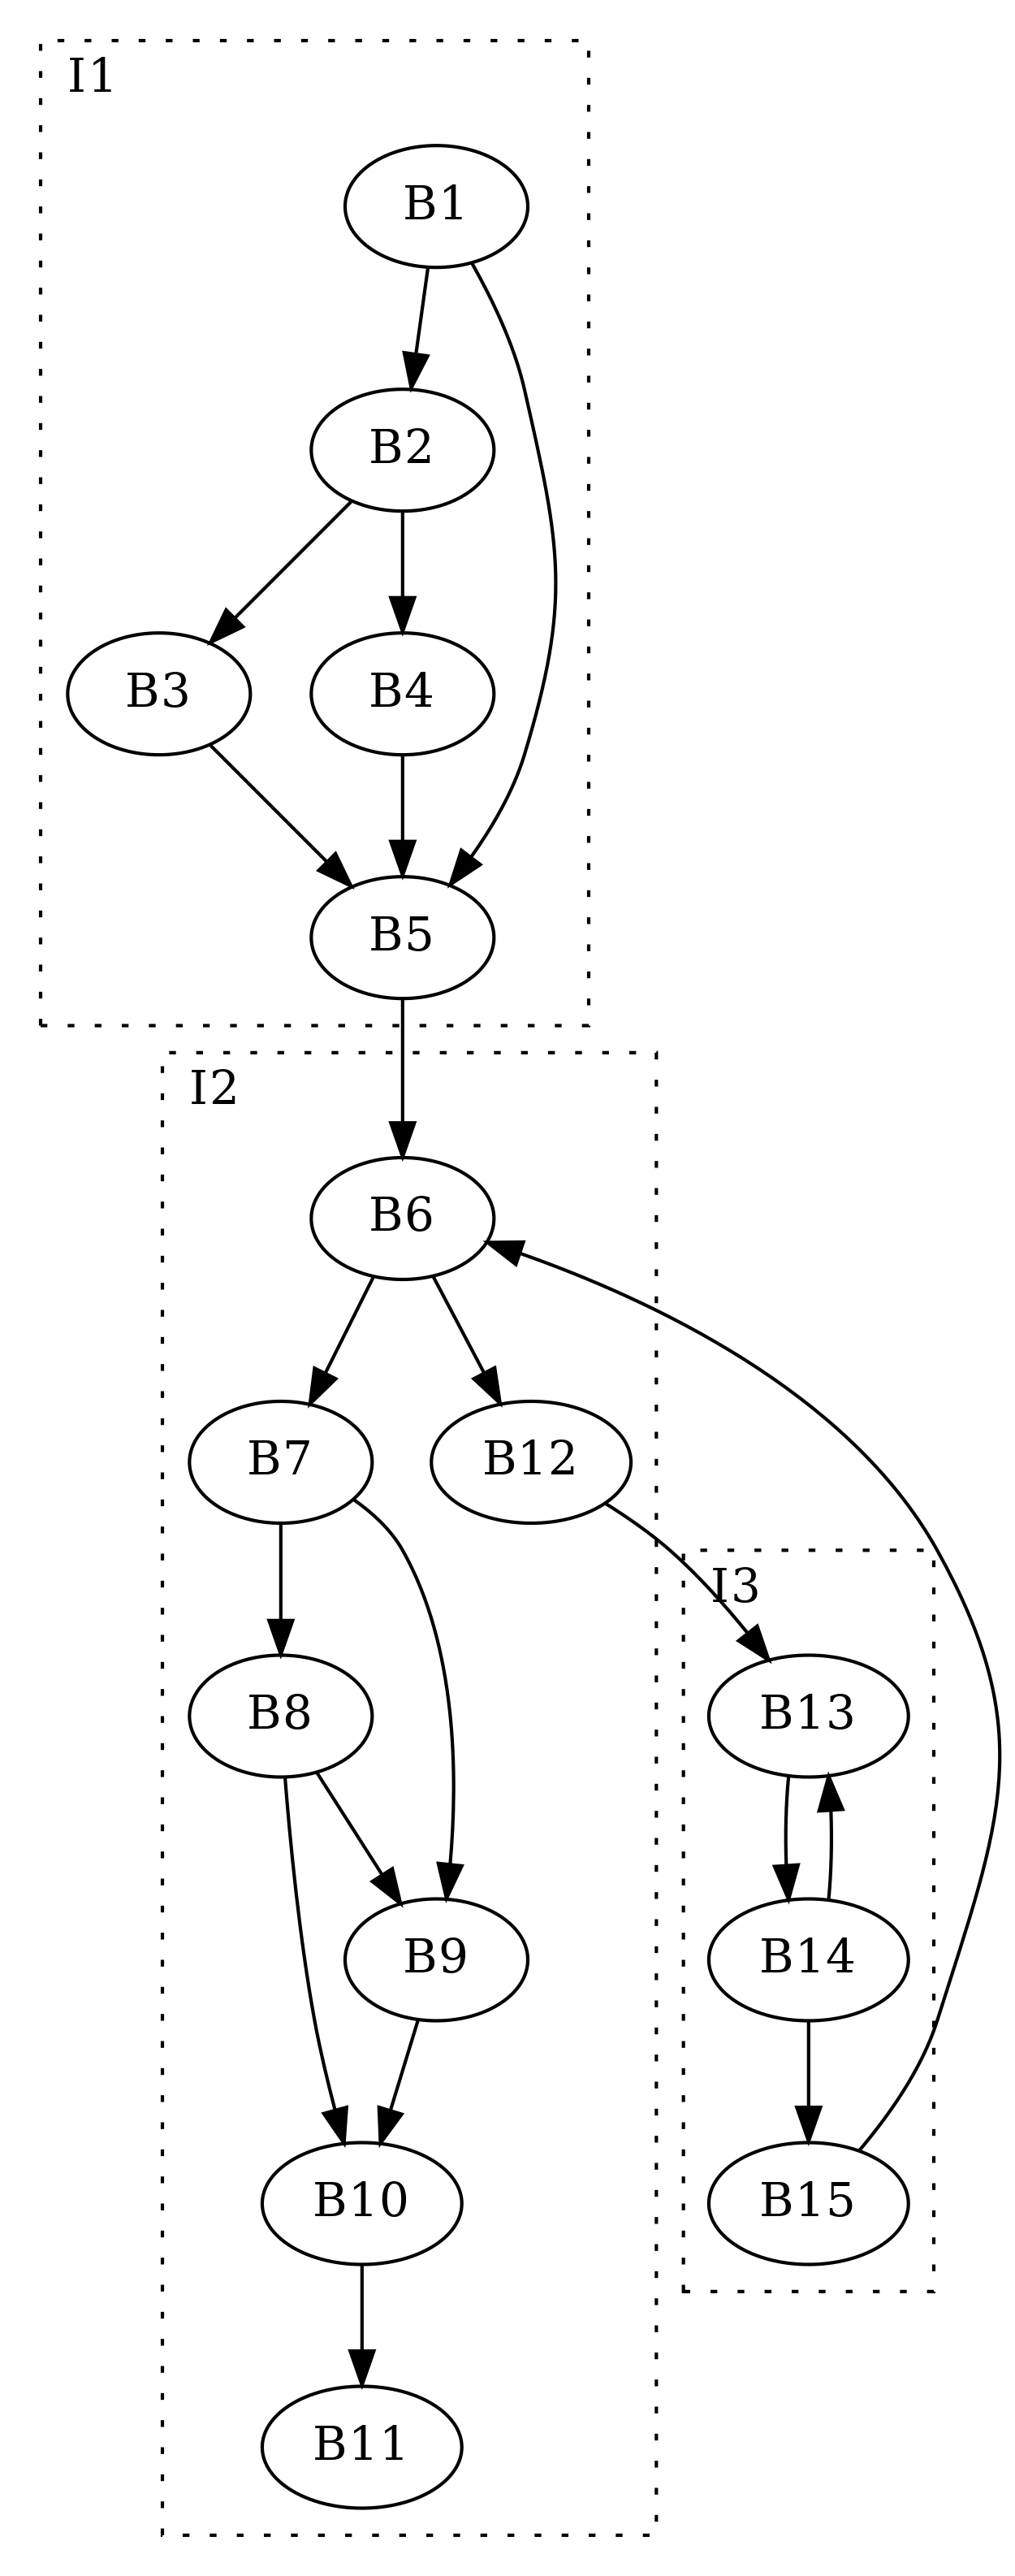
\includegraphics[width=\textwidth]{inc/3_background/interval_method/derived_sequence_of_graphs/G_1.png}
		\caption{$G^1$}
	\end{subfigure}
	\qquad
	\begin{subfigure}[b]{0.12\textwidth}
		\centering
		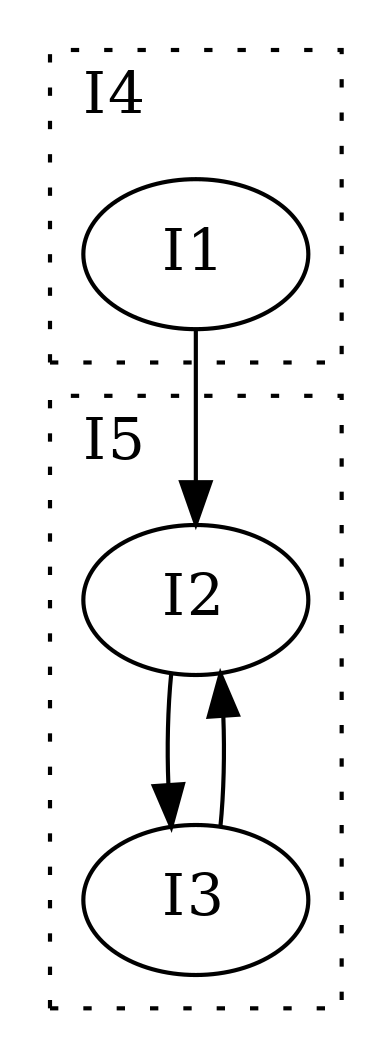
\includegraphics[width=\textwidth]{inc/3_background/interval_method/derived_sequence_of_graphs/G_2.png}
		\caption{$G^2$}
	\end{subfigure}
	\qquad
	\begin{subfigure}[b]{0.12\textwidth}
		\centering
		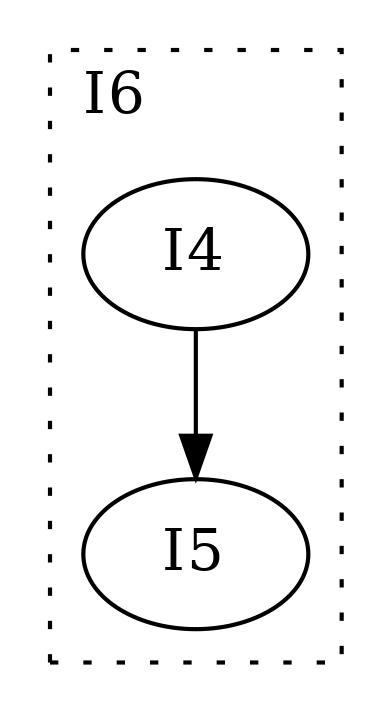
\includegraphics[width=\textwidth]{inc/3_background/interval_method/derived_sequence_of_graphs/G_3.png}
		\caption{$G^3$}
	\end{subfigure}
	\qquad
	\begin{subfigure}[b]{0.08\textwidth}
		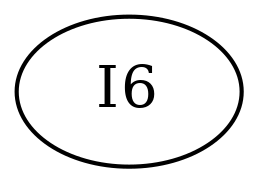
\includegraphics[width=\textwidth]{inc/3_background/interval_method/derived_sequence_of_graphs/G_4.png}
		\vspace{2em}
		\caption{$G^4$}
	\end{subfigure}
	\caption{Derived sequence of graphs, $G^1, ..., G^n$; adapted from figure 3 of C. Cifuentes' \textit{Structuring Decompiled Graphs} \cite{structuring_decompiled_graphs}.}
	\label{fig:derived_sequence_of_graphs}
\end{figure}

% ~~~ [ Back Edge ] ~~~~~~~~~~~~~~~~~~~~~~~~~~~~~~~~~~~~~~~~~~~~~~~~~~~~~~~~~~~~

%\subsubsection{Back Edge}

%\todo{TODO: define Back Edge}

% ~~~ [ Reverse Post-order ] ~~~~~~~~~~~~~~~~~~~~~~~~~~~~~~~~~~~~~~~~~~~~~~~~~~~

%\subsubsection{Reverse Post-order}

%\todo{TODO: define Reverse Post-order}
